% !TeX spellcheck = es_ES

\documentclass[twocolumn,10pt]{article}
\usepackage[utf8x]{inputenc}
\usepackage[spanish]{babel}
\usepackage[a4paper,top=2cm,bottom=2cm,left=2cm,right=2cm,marginparwidth=1.75cm,headheight=28pt]{geometry}
%Letra general
\usepackage{mathastext}
\usepackage{IEEEtrantools}

\renewcommand{\familydefault}{\sfdefault}
\usepackage[scaled=1]{helvet}
\usepackage[format=plain,
            labelfont={bf,it},
            textfont=it]{caption}
\usepackage{color}
\usepackage{fontawesome,graphicx}
\usepackage{siunitx}
\usepackage{booktabs,tabularx,makecell,multirow,caption}

%Math
\usepackage{amsmath}
\usepackage{amsfonts}

%commands
\newcommand{\glossentry}[2]{$#1$\indent #2 \par \vspace{.4cm} } %Entradas para glosario
\newcommand{\glossml}[3]{$#1$\indent #2 \emph{#3}  \par \vspace{.4cm} } %Entradas para glosario

\newcommand{\bigpar}[1]{\bigg(
#1 \bigg) }
\newcommand{\dprime}{ {\prime \prime} }
\newcommand{\di}{\textrm{d}}
\newcommand{\tprime}{ {\prime \prime \prime} }
\newcommand{\fit}{\textit{\textrm{f }}}
\newcommand{\corr}{{\textrm{\color{red} Revisar}}}
\newcommand{\Kf}[1]{ K_{\textit{\textrm{f}}_{\textrm{#1}}} }
\newcommand{\Kfs}[1]{ K_{\textit{\textrm{fs}}_{\textrm{#1}}} }
\newcommand{\siga}[1]{ \sigma_{{\textrm{a}}_{\textrm{#1}}} }
\newcommand{\sigm}[1]{ \sigma_{{\textrm{m}}_{\textrm{#1}}} }
\newcommand{\pe}{\textit{\textrm{p}}}
\newcommand{\gut}{{\color{green}\faCheck}}
\newcommand{\HC}{$H_xC_y$}
\newcommand{\NX}{$NO_x$}
\begin{document}
\title{Resumen de Motores a Combustión interna}

\twocolumn[
\centering 
{ \bf \LARGE Resumen de Finanzas \par}
\vspace{.2cm}
{\sc \large Patricio Whittingslow\par }
\vspace{.4cm}
]
\glossml{A}{Activos.}{Assets}
\glossml{P}{Pasivos.}{Liabilities}

\glossml{PN}{Patrimonio neto.}{Equity (commonly used for companies) or net worth (individuals)}

\glossml{V}{Ventas.}{Revenue}

\glossml{Q}{Cantidad demanda.}{Quantity demanded}

\glossml{VF}{Valor futuro.}{Future value $(FV)$}
\glossml{VP}{Valor presente/actual.}{Principal/present value $(PV)$}
\glossml{VA}{Valor actual. Refiere los flujos positivos y negativos a un mismo punto en el tiempo para evaluar la conveniencia del proyecto.}{Present value (PV)}

\glossml{VAN}{Valor actual neto}{Net present value $(NPV)$}

\glossml{TREMA}{Tasa de rendimiento mínima aceptable.}{Minimum acceptable rate of return $(MARR)$}

\glossml{r,i}{Tasa de descuento \& tasa de interés.}{Discount rate}



\glossml{g}{Tasa de crecimiento.}{Growth rate}

\glossml{TIR}{Tasa interna de retorno.}{Internal rate of return (a type of discount rate) $(IRR)$}

\glossml{TEM}{Tasa efectiva mensual.}{Effective monthly interest rate}

\glossml{TET}{Tasa efectiva trimestral (cada 3 meses).}{}
\glossml{PN}{Patrimonio Neto.}{}
\glossml{TEA}{Tasa efectiva anual.}{Effective annual interest rate}
\glossml{CPI}{}{Consumer price index.}
\glossml{\pi=\frac{\di CPI}{\di t}}{Inflación.}{Rate of inflation.}
\glossml{FEO}{Flujo efectivo ordinario.}{Free cash flow from operations or operating free cash flow $(FCFO)$}
\glossml{FEE}{Flujo efectivo extraordinario.}{}
\glossml{UAIG=UB}{Utilidad antes de impuestos a las ganancias o utilidad bruta.}{Profit before tax $(PBT)$}
\glossml{UN}{Utilidad neta o utilidad despues de impuestos a las ganancias.}{Net income, net profit, bottom line or net earnings $(NI)$}
\glossml{G}{Ganancias o beneficio.}{Earnings}
\glossml{IG}{Impuestos a las ganancias.}{Income tax $(IT)$}
\glossml{BU}{Bienes de uso.}{Durable goods}

\glossml{VL}{Valor en libros.}{Carrying value/amount or book value.}
\glossml{K_T}{Capital de trabajo.}{Capital goods}
\glossml{K_S}{Capital Social.}{Social Capital}

\glossml{EBT}{Ganancias antes de impuestos.}{Earnings before tax.}
\glossml{EBIT}{Ganancias antes de interés y impuestos.}{Earnings before interest \& tax.}
\glossml{EBITDA}{Ganancias antes de interés, impuestos, depreciación y amortización.}{Earnings before interest, tax, depraciation \& amortization.}
\glossml{CV}{Costos variables.}{Variable costs}
\glossml{CF}{Costos fijos.}{Fixed costs}
\glossml{CT}{Costos totales.}{Total costs}
\glossml{CT_{Me}}{Costo total promedio.}{Total cost average}

\glossml{PER}{Relación precio-beneficio.}{Price to earning ratio.}


\newcommand{\fiN}{\ensuremath{f_i^N}}

\tableofcontents

\newpage
\part{Primer Parcial}
\subsection{Crecimiento económico}
% TODO: \usepackage{graphicx} required
\begin{figure}[htb!]
	\centering
	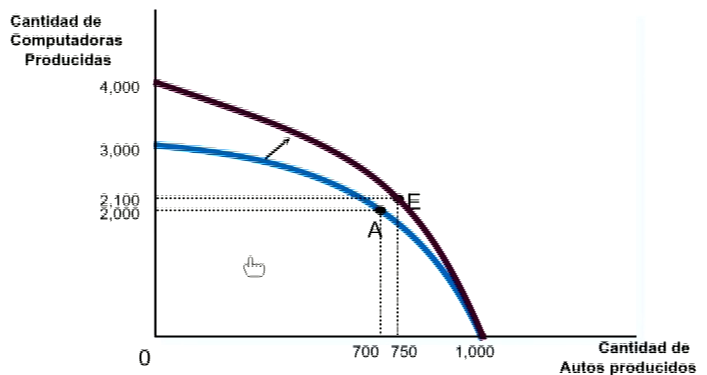
\includegraphics[width=1\linewidth]{fig/frontProd}
	\caption{Frontera de producción. Se visualiza crecimiento econ\'omico como el cambio de la curva. En este caso hubo crecimiento en la industria de computadoras. Notar que tambi\'en aumento la cantidad de autos producidos para un mismo r\'egimen de producci\'on! El mayor aprovechamiento de recursos ocurre sobre el punto medio (dado que es una curva concava para el origen y simetrica sobre $y=x$).}
	\label{fig:frontprod}
\end{figure}

\subsection{Costos de oportunidad}

Cuando uno opta por un proyecto o hace una compra hay un costo de oportunidad. Es decir, la plata que uno usa para comprar una bebida tiene un costo asociado ya que no se puede usar para comprar un sándwich.

Ejemplo con una empresa: optar por vender medialunas conlleva un costo de oportunidad porque dejaste de un lado usar la harina para vender pan.

\subsection{An\'alisis marginal}
Una persona toma una decisión \textbf{racional} si y s\'olo si el beneficio marginal es superior al costo marginal. El costo marginal es el costo de producir una unidad m\'as.

Utilidad: Capacidad que tiene un bien para satisfacer lasa necesidades humanas

Utilidad Marginal: Utilidad que proporciona la \'ultima unidad pose\'ida de un bien. Ello comporta que cuanto m\'as escaso sea un bien mayor sea el valor que le otorgamos. 

Ejemplo muerto de sed en el desierto. La utilidad marginal del primer vaso de agua va ser mayor al quinto vaso de agua.
\section{Curva de la demanda}
Los resultados de las decisiones de los individios que act\'uan como \textit{consumidores} en el mercado se expresan en una \textit{demanda de mercado}. La demanda de mercado es la suma de demandas individuales. La demanda relaciona precio y cantidad demandada.

La demanda depende de la renta, las expectativas,

En general tiene pendiente decreciente. A mayor precio, menor cantidad demandada (precio en eje $y$)
\begin{description}
	\item[Bienes normales] Si la renta aumenta, la demanda aumenta
	\item[Bienes inferiores] Si la renta aumenta, la demanda disminuye
	\item[Bienes complementarios] La relación entre la demanda del bien $X$ y del precio de $C_X$ es inversa tal que si aumenta el precio del bien complementario $C_X$ de $X$, entonces se reducirá la cantidad demandada de $X$ (Automóvil $X$ vs. gasolina $C_X$)
	\item[Bienes sustitutos] Si aumenta el precio del bien sustituto $S_X$ se reduce la cantidad demandada de $S_X$ y por lo tanto aumenta la demanda de $X$. La relación entre la demanda de $X$ y del precio de $S_X$ es directa (Hellmann's vs. Heinz) 
\end{description}

\section{Curva de la oferta}

En general tiene pendiente creciente: a mayor precio, mayor cantidad ofrecida

Depende de costos de fabricaci\'on, de la tecnolog\'ia del ofreciente, el ambiente político o econ\'omico (especulaci\'on de precios futuros o fluctuaciones en el mercado).

\begin{figure}[htb!]
	\centering
	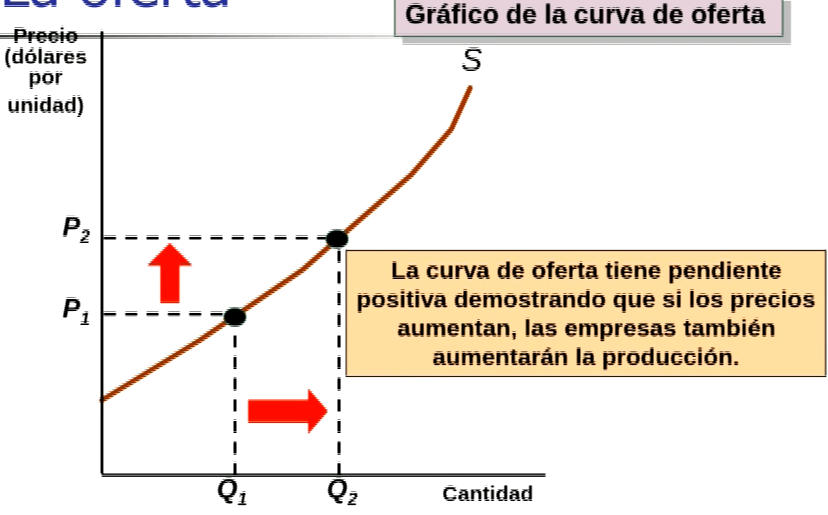
\includegraphics[width=1.0\linewidth]{fig/la_oferta}
	\caption{Los costos marginales son crecientes, a esto se debe la forma de la curva de oferta. Esto tambi\'en significa que va llegar un punto a partir del cual no conviene vender m\'as. La curva de demanda es la suma de todas las demandas individuales del mercado. Esto se puede visualizar con el siguiente ejemplo: a medida que aumenta el precio, va haber m\'as empresas que pueden entrar al mercado para ofrecer el producto.}
	\label{fig:laoferta}
\end{figure}

\subsection{Precios}
Precio nominal y real.

Ejemplo nafta: El precio nominal es el que est\'a escrito en el surtidor de nafta. Si hablamos de precios reales se tiene que hablar del momento en el tiempo. Si en el 2020 la nafta vale 60\$ y en el 2015 val\'ia 15\$ hay que transformar el precio del 2015 al precio real (precio 2020). Para esto se multiplica el precio nominal del 2015 por el cociente 
\[
\text{Precio real de la nafta en el 2015}=15\$\cdot \frac{IPC_{2020}}{IPC_{2015}}
\]
donde $IPC$ es el indice de precio consumidor para el a\~no.

\subsection{Eficiencia Pareto}
No se puede hacer cambios a un mercado en equilibrio para mejorar la situación de algunos sin empeorar la situación para otros. 

Es decir: un mercado sin intervenci\'on de estado ni fijaci\'on de precios es eficiente.


\section{Elasticidad}

Para hacer análisis de ``que pasa con la cantidad demandada si hacemos $x$''. Las elasticidades tienen la forma
\[
\eta = \frac{\text{Efecto}}{\text{Est\'imulo}}
\]
y dependen de existencia de sustitutivos cercanos, si son bienes necesarios o de lujo, definición del mercado, el horizonte temporal, y la proporción del gasto total que se gasta en ese bien. Ejemplo de demanda inel\'astica: medicamentos críticos como insulina. Los endulzantes son un ejemplo de un mercado elástico.

La \textbf{elasticidad (de la demanda)} $\eta$ es la variación porcentual de la cantidad demandada sobre la variación porcentual del precio.
\begin{IEEEeqnarray*}{c}
\eta = \left| \frac{\Delta Q / Q}{\Delta P / P} \right|= \left| \frac{P\times \Delta Q}{Q \times \Delta P} \right|
\end{IEEEeqnarray*}
también existe la elasticidad de punto $\eta = \left| \frac{\di Q}{\di P}\cdot\frac{P}{Q} \right|$. Algunas fuentes expresan la elasticidad sin el modulo.

\begin{description}
	\item[$\eta_p> 1$] Demanda elástica
	\item[$\eta_p = 1$] Demanda de elasticidad unitaria (ganancia máxima)
	\item[$\eta_p < 1$] Demanda inelástica
\end{description}

\textbf{Elasticidad ingreso} o renta de la demanda $e$ es la variación porcentual de la cantidad demandada sobre el cambio porcentual en la renta o ingreso del consumidor.
\begin{IEEEeqnarray*}{c}
e = \frac{ \Delta Q / Q }{ \Delta Y / Y }
\end{IEEEeqnarray*}

\begin{description}
	\item[$e>1$] Bien de lujo
	\item[$0<e<1$] Bien básico
	\item[$e>1$] Bien inferior
\end{description}


Luego se tiene la \textbf{elasticidad cruzada de la demanda} $\eta_{XY}$ que es la variación de la cantidad demandada de $X$ sobre la variación porcentual del precio de $Y$.

\begin{IEEEeqnarray*}{c}
\eta_{XY} = \frac{\Delta Q_X / Q_X}{\Delta P_Y / P_Y}
\end{IEEEeqnarray*}

\begin{description}
	\item[$e_{XY} > 0$] Bienes sustitutos
	\item[$e_{XY} < 0$] Bienes complementarios
\end{description}


La \textbf{elasticidad precio de la oferta} $\varepsilon_p$ se calcula como la variación porcentual de la cantidad ofrecida sobre la variación porcentual del precio
\begin{IEEEeqnarray*}{c}
 \varepsilon_p = \frac{\Delta \% Q_O}{ \Delta \% P}
\end{IEEEeqnarray*}

Si se habla de la \textbf{elasticidad precio de la demanda} se reemplaza $Q_O$ por $Q_S$.
\subsection{Excedente y escasez del consumidor}

Los puntos de la curva de demanda muestran la valoraci\'on m\'axima que el consumidor da a cada cantidad de bien (i.e. lo que estar\'ia dispuesto a pagar por esa cantidad). El precio de mercado se determina por el curce entre la oferta y la demanda, y representa la valoraci\'on del bien por parte del consumidor marginal (i.e. lo que el consumidor menos intersado estar\'ia dispuesto a pagar como m\'aximo por el bien).

La diferencia entre la curva de demanda y el precio es el \textbf{excedente del consumidor}. Esto es el valor adicional que los consumidores estar\'ian dispuestos a pagar por  el bien, pero como no deben pagarlo lo ganan.

\begin{figure}[tbh!]
	\centering
	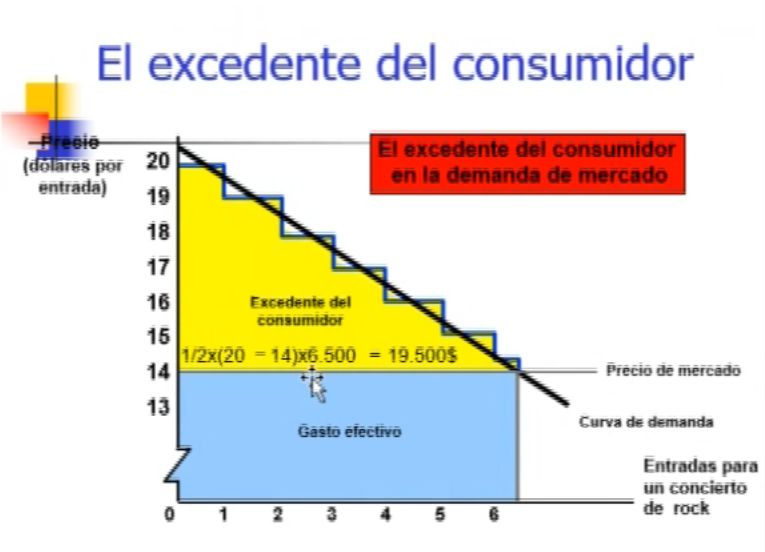
\includegraphics[width=1\linewidth]{fig/excedentConsumidor}
	\caption{Ejemplo: Viene nuestra banda de rock favorita. Estamos dispuestos a pagar 20 por la primer entrada, 19 por la segunda, etc; pero como hay un solo precio de mercado no ``ahorramos'' lo que esta en amarillo.}
	\label{fig:excedentconsumidor}
\end{figure}

\begin{figure}[tbh!]
	\centering
	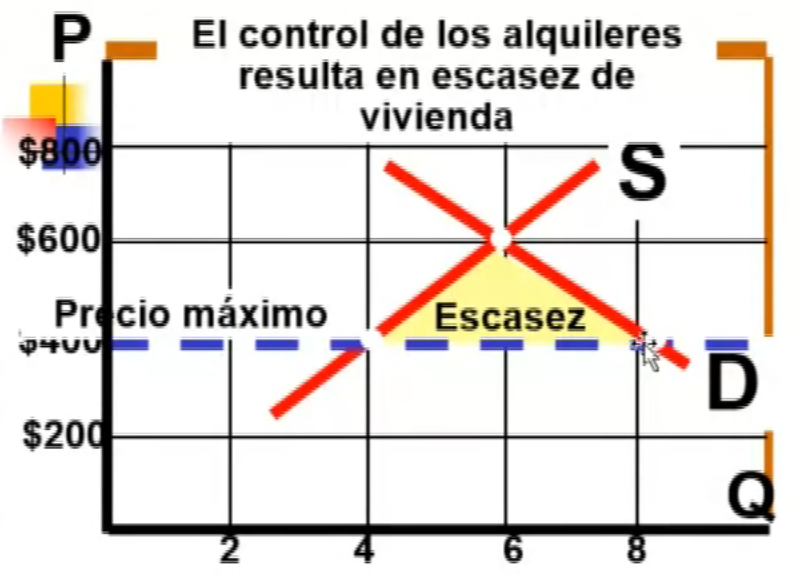
\includegraphics[width=1\linewidth]{fig/escasezConsumidor}
	\caption{Se fija un precio m\'aximo por debajo del punto de equilibrio (para que tenga efecto). Luego los consumidores van a demandar una cantidad 8 y los productores van a encontrarse teniendo que vender 4 unidades para maximizar beneficio. Se produce escasez del bien.}
	\label{fig:escasezconsumidor}
\end{figure}


\begin{figure}[tbh!]
	\centering
	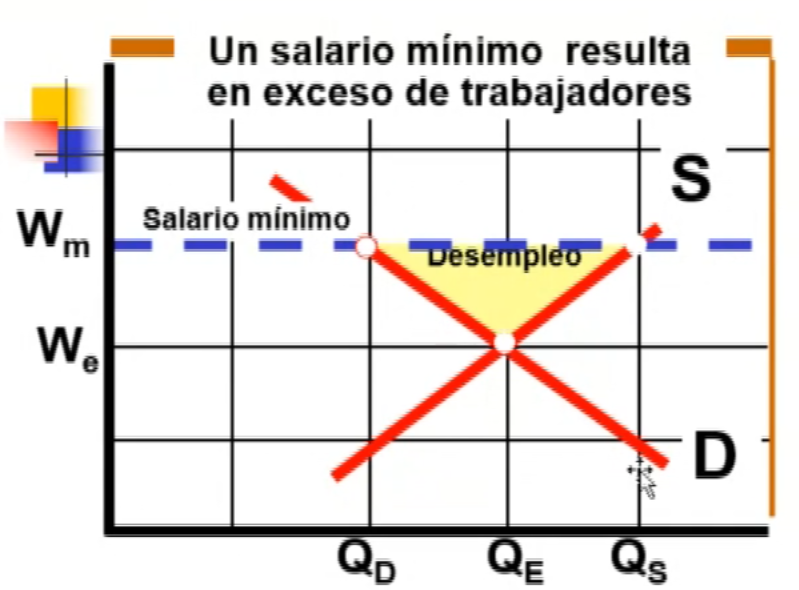
\includegraphics[width=1\linewidth]{fig/escasezProductor}
	\caption{Se fija un salario m\'inimo por arriba del punto de equilibrio. Las empresas estar\'an buscando disminuir su capital laboral para reducir costos produciendo as\'i desempleo.}
	\label{fig:escasezproductor}
\end{figure}



\section{Función de la producción}
La función de la producción usa dos factores (Trabajo $L$ y capital $K$) y puede diferir según el plazo de análisis $\Delta t$.
\[
Q = f(K,L, \Delta t)
\]

Un ejemplo puede ser una simplificaci\'on de una pizzer\'ia. Se tiene cantidad de trabajo $L$ (pizzeros), cantidad de capital $K$ (hornos).

\begin{table}[tbh!]
	\centering
	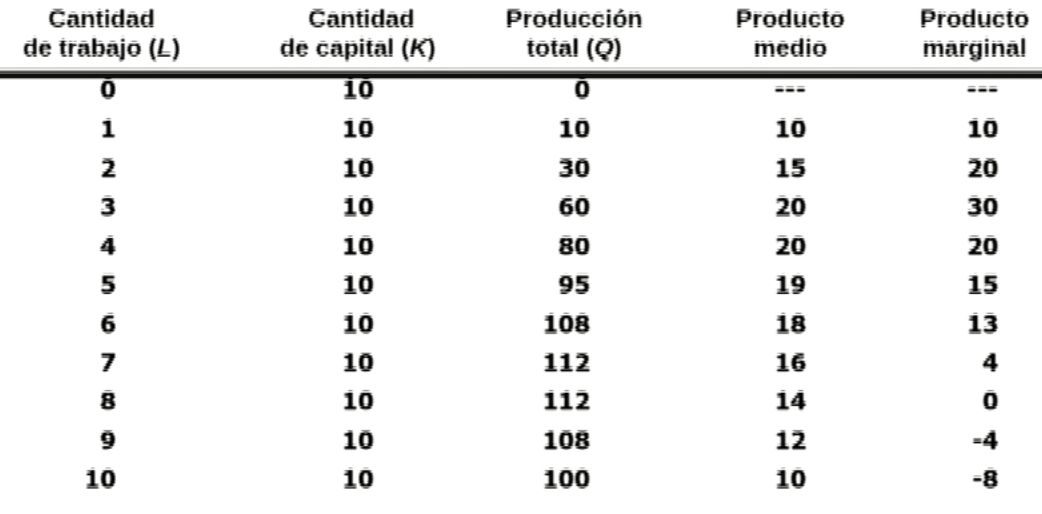
\includegraphics[width=1\linewidth]{fig/funcionProduccionTabla}
	\caption{Contratando los primeros pizzeros se aumenta la producci\'on fuertemente. Después del sexto pizzero empieza a caer el rendimiento hasta que es nocivo tener tantos pizzeros en un solo restaurante. Antes de agregar el octavo pizzero se necesita ampliar el local (agregar capital $K$ en forma de hornos en este ejemplo). Esto es un ejemplo a corto plazo: se mantiene constante uno de los factores de producci\'on: $K$.}
	\label{fig:funcionproducciontabla}
\end{table}


\begin{description}
	\item[Corto plazo] El lapso más largo durante el cual no es posible alterar al menos unos de los factores de producción
	\item[Largo plazo] El lapso más corto necesario para alterar todos los factores involucrados en el proceso productivo
\end{description}

\begin{figure}[tbh!]
	\centering
	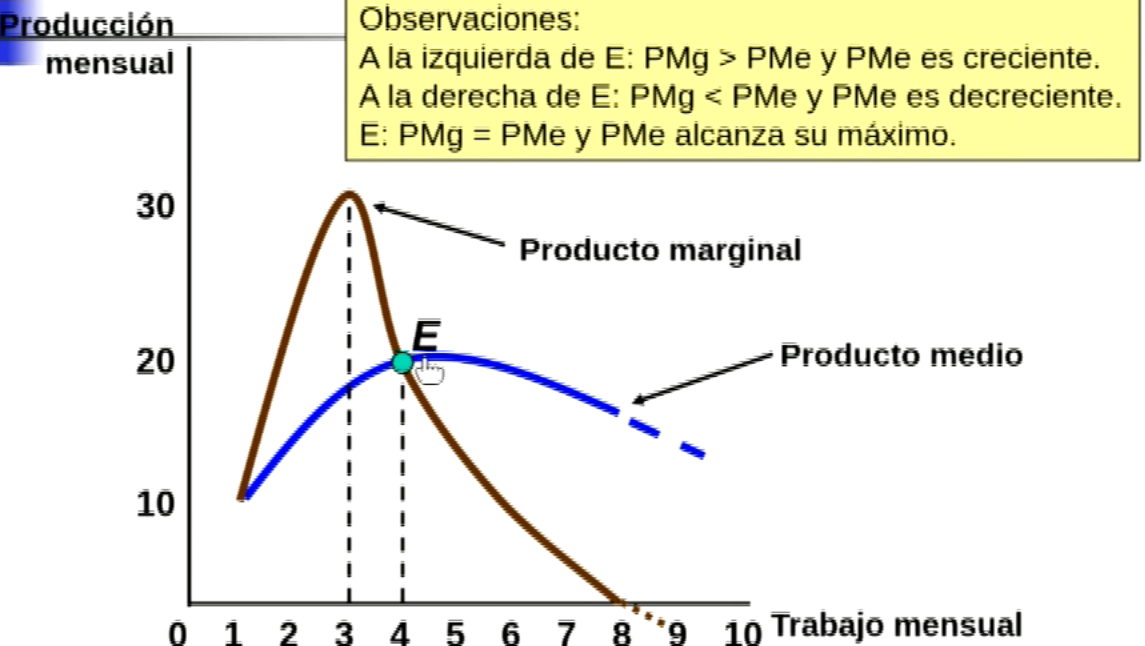
\includegraphics[width=1\linewidth]{fig/funcionProduccionLvar}
	\caption{La producci\'on con trabajo $L$ variable. Note que el producto medio m\'aximo se alcanza cuando este coincide con el producto marginal.}
	\label{fig:funcionproduccionlvar}
\end{figure}



\subsection{Ley de los rendimientos marginales decrecientes}
En el corto plazo hay un factor fijo (suele ser $K$) y uno variable (suele ser $L$). Esta ley establece que a medida que se incorporan unidades del factor variable al factor fijo, el rendimiento de cada unidad adicional es menor a partir de cierta cantidad límite.

Esto se debe a que se va saturando el factor fijo con respecto al factor variable. En el ejemplo de la pizzería se saturaban los hornos.

 \subsubsection{Addendum: Teor\'ia de Malthus}
Thomas Malthus predijo alrededor de 1800s que por la ley de rendimientos marginales decrecientes iba a haber una escasez de comida por la sobrepoblaci\'on debido a que se iba a necesitar una gran cantidad de personal para cosechar/orde\~nar etc. Malthus no tuvo en cuenta a la tecnolog\'ia, la cual aument\'o la producci\'on por unidad de trabajo.

\begin{figure}[tbh!]
	\centering
	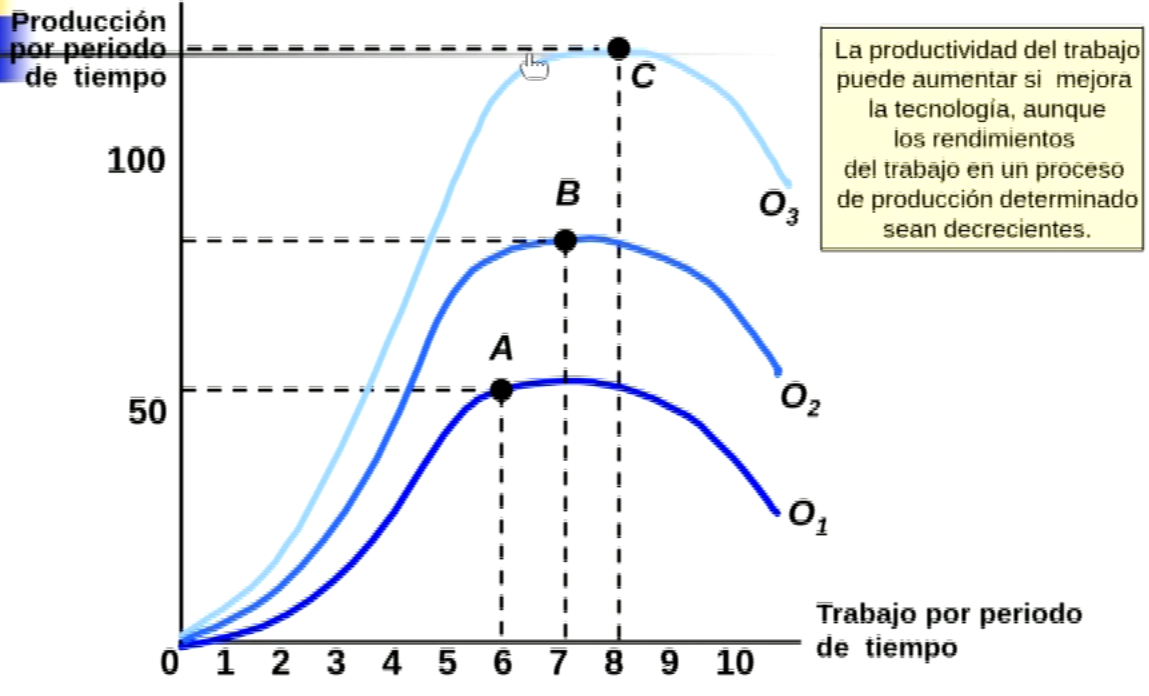
\includegraphics[width=1\linewidth]{fig/efectomejoratecnologiaMalthus}
	\caption{El efecto de la tecnolog\'ia sobre la funci\'on producción}
	\label{fig:efectomejoratecnologiamalthus}
\end{figure}

\section{Costos}

Todo costo es un costo de oportunidad ya que al desembolsar se gasta la oportunidad de usar el dinero para otro fin. Los costos explícitos son los que se pagan de manera directa: pago por hora hombres, amortizaciones, por materia prima y no incluyen los costos por comparaci\'on con otras alternativas (costos de oportunidad).

Se puede tambi\'en categorizar los costo

\section{Mercados}
\subsection{Control externo}

En un mercado se tiene el consumidor con su curva de demanda ($Q_D$) y el vendedor/empresa/ofreciente con su curva de oferta ($Q_O$ o a veces denotado con sub\'indice $S$ por el ingl\'es \emph{supply}) en funci\'on del precio $P$.

Cuando se subsidia un producto pagando al vendedor el punto de equilibrio cambia seg\'un
\[
Q_O(P^{*}+\text{subsidio}) = Q_D(P^{*}) 
\]

Cuando se paga al consumidor pr unidad adquirida se tiene

\[
Q_D(P^{*}-\text{subsidio}) = Q_O(P^{*}) 
\]

\subsection{Competencia perfecta}
En una competencia perfecta se hacen las siguientes suposiciones
\begin{itemize}
	\item Productos homogeneos
	\item Empresas Precio-aceptantes
	\item Información perfecta
\end{itemize}

El mercado de competencia perfecta está en equilibrio cuando:


\begin{itemize}
	\item El precio de mercado es único
	\item La oferta es igual a la demanda
	\item Todos los consumidores maximizan la utilidad
	\item Todas las empresas maximizan el beneficio
\end{itemize}

Decisiones de producción:
\begin{itemize}
	\item Como ya vimos, los beneficios se maximizan cuando $I_{Mg}=C_{Mg}$
	\item Si el $P>CT_{Me}$, la empresa obtiene beneficios
	\item $CV_{Me}<P<CT_{Me}$, la empresa incurre en pérdidas
	\item $P<CV_{Me}<CT_{Me}$, la empresa debe cerrar
\end{itemize}
%\part{Segundo Parcial}
\section{Contabilidad}

\textbf{Empresa.} Organismo que coordina factores productivos destinados a producir e intercambiar bienes y servicios en la sociedad. Realiza compras, pagos, rentas, cobros, transforma insumos para obtener nuevos bienes y servicios. 

\textbf{Contabilidad} Registro ordenado y cronológico de hechos económicos (uso de recursos).

Los \textbf{pasivos} incluyen deudas y obligaciones con terceros. \textbf{Activos} incluye bienes y derechos de la empresa

 \textbf{Patrimonio Neto} incluye aporte de socios y ganancias acumuladas menos dividendos repartidos. Es el valor contable que pertenece a accionistas, equivalente a los aportes de los socios a lo largo durante la vida de la empresa.

\subsection{El balance}

Ecuación patrimonial: 
\[
A = P + PN
\]

\begin{table}[h!]
	\centering
	\begin{tabular}{cc}
		\multirow{4}{*}{\shortstack[c]{\textbf{Activos}\\ \underline{Corriente}\\Caja y básicos\\ Inversiones y financiamientos\\Bienes de cambio\\Creditos por ventas\\ \underline{No Corriente}\\Bienes de uso\\Inversiones}} & \textbf{Pasivo} \\ 
		 & \shortstack[c]{\underline{Corriente}\\Deudas comerciales\\Deudas bancarias CP\\ \underline{No Corriente}\\Deudas bancarias LP} \\
		& \textbf{Patrimonio Neto} \\
		 & \shortstack[c]{Capital\\Utilidades\\Reservas}
	\end{tabular}
\end{table}

Términos de contabilidad:
\begin{description}
	\item[Caja y bancos"".] Efectivo, cheques, valores e rápida liquidación.
	\item[Inversiones corrientes.] Liquidaciones antes de 1 año.
	\item[Inversiones no corrientes.] Liquidaciones en mas de 1 año.
	\item[Bienes de cambio] Productos terminados. En recesión aumenta (disminuyen ventas, se acumula stock). En demanda disminuye.
	\item[Creditos por ventas] Lo que los clientes deben por mercaderia u otros conceptos a pagar en $<$ 1 año
	\item[Bienes de uso.] Maquinaria, equipos, vehiculos, edificios. Es igual al costo menos las amortizaciones acumuladas (pérdida de valor)
	\item[Deudas comerciales.] Contraídas con los proveedores
	\item[Fondo de maniobra o Capital de Trabajo.] La parte del activo que permanece. $K_T=$Pasivo no corriente + PN - Activo no corriente
	\item[Capital de trabajo operativo]  Necesidades operativas de fondo. Activos corrientes operativos - Pasivos corrientes operativos.
\end{description}

Calculo de amortizaciones:
\[
A = \frac{\text{Valor Original - Valor residual contable}}{\text{Vida útil}}
\]

\begin{table}[h]
	\centering
	\begin{tabular}{|l|} \hline
		+ Ingresos por ventas \\
		- Costos variables (``de ventas") \\ \hline
		= Utilidad bruta \\
		- Costos fijos (``Administración y ventas") \\ \hline
		= EBITDA \\
		- Amortizaciones \\ \hline
		= EBIT \\
		- Intereses \\ \hline
		= EBT \\
		- Impuestos a las ganacias
		\\ \hline
		= Utilidad Neta\\ \hline
	\end{tabular}
\caption{Cuadro de resultados}
\end{table}


\subsection{Flujo de caja. \textit{Cash flow}}

\[
A=P+PN\rightarrow \Delta A = \Delta P + PN \rightarrow \Delta C = \Delta P + \Delta PN - \Delta A
\]
donde $\Delta C$ es el flujo de fondos total.


\begin{IEEEeqnarray*}{rCl}
\Delta C &=& \Delta D_{comerc} + \Delta D_{financ} + Utilidades + Aportes \\
& & - Dividendos -(\Delta Cred + \Delta BC + \Delta BU)
\end{IEEEeqnarray*}
donde $\Delta BU$ es la inversión menos la amortización.

\begin{IEEEeqnarray*}{rCl}
	\Delta C &=& \overbrace{EBIT(1-a) + Amort. - \Delta Cred. - \Delta BC + \Delta D_{com}}^{=FFO} \\
	& & \underbrace{-Invers.}_{=FFI} + \underbrace{\Delta D_{fin} + Aport. - Div. Inter(1-a)}_{=FFF}
\end{IEEEeqnarray*}
entonces la variación de caja (lo que representa el cash que entró y salió de la empresa en un periodo determinado) se puede escribir como
\[
\Delta C = FFO + FFI + FFF
\]
\subsection{Valor de mercado vs. valor de libro}

\begin{description}
	\item[Valor de libro.] Valor contable oficial de los activos y del capital de los accionistas. Valor de libro por acción = $\frac{PN}{Nro~de~acciones}$
	\item[Valor de mercado.] Incluye cosas que el valor de libro no, como todos los activos y pasivos de la empresa, los activos estan valuados a costos de adquisicion menos amortizaciones acumuladas.
\end{description}

\subsection{Principio de lo devengado}

Las ventas se devengan independientemente de si se cobran o no. Los costos de devengan independientemente de si se pagan o no.

\subsection{Principio de partida doble}

\begin{table}[h!]
	\centering
	\begin{tabular}{c|c}
		Debe & Haber \\ \hline
		$\uparrow$ Activo &$\uparrow$ Pasivo \\
		$\downarrow$ Pasivo & $\uparrow$ PN \\
		$\downarrow$ PN & $\downarrow$ Activo \\ \hline
		Saldo Deudor & Saldo Acreedor 
	\end{tabular}
\caption{$\sum debe = \sum haber$}
\end{table}
\[
Activo + Perdidas = Pasivo + K_S + Ganancias 
\]
\[
PN = K + Utilidades
\]
donde $Utilidades = Ganancias + Perdidas$

\subsection{Tipos de cuentas}
\begin{description}
	\item[Patrimoniales] Reflejan los componentes del patrimonio
	\begingroup
	\small
	\begin{description}
		\item[Del activo.] Bienes tangibles o no a favor de la empresa
		\item[Del pasivo.]  Deudas y obligaciones de la empresa
		\item[Del PN] Pueden ser de \textbf{Capital} (aporte de los socios) o  \textbf{Utilidades Acumulados} (resultados de la empresa)
	\end{description}
\endgroup
\item[De Resultados.] Positivos o negativos. Variaciones de resultados
\item[Regulariadores.] Activo, pasivo o PN. Llevan el valor de las cuentas que están corrigiendo un importe más cercano a ser realidad económica""
\end{description}

\section{Indices financieros}

\subsection{Liquidez}
La liquidez es de interes a los proveedores, sobre todo los que prestan dinero o CP a la empresa

\begin{description}
	\item[ILC] Índice de liquidez corriente $=\frac{AC}{PC}$
	\item[ILS] Índice de liquidez seco $=\frac{AC-BC}{PC}$
	\item[ILA] Índice de liquidez absoluto $=\frac{AC-BC-C}{PC}$
\end{description}

\subsection{Rentabilidad}
\begin{description}
	\item[ROE] Rentabilidad del PN $=\frac{UN}{PN}$
	\item[ROA] Rentabilidad operativa $=\frac{EBIT}{A}$
	\item[Márgen(sobre las rentas)]:
	\begingroup
	\small
	\begin{description}
		\item[Bruto] $=\frac{UB}{V}$
		\item[Operativo] $=\frac{EBIT}{V}$
		\item[Neto] $=\frac{UN}{V}$
	\end{description}
	\endgroup
\end{description}
El accionista esta interesado en el márgen neto. 
\subsection{Operativos}
\begin{description}
	\item[PMC] Plazo medio de cobranzas $=\frac{Creditos}{V/360}[dias]$
	\item[Liquidez de inventarios]  $=\frac{BC}{Costo~Ventas/360} [dias]$
	\item[PPPP] Plazo promedio de pago a proveedores $=\frac{Deuda~Comercial}{Costos~Ventas/360}[dias]$ 
	\item[Rotación] description
	\begingroup
	\small
	\begin{description}
		\item[de BC] $=\frac{Costo~Ventas}{BC}[1/a\tilde{n}o]$
		\item[de Activos] $=\frac{V}{A}[1/a\tilde{n}o]$
	\end{description}
	\endgroup
\end{description}

\subsection{Endeudamiento}
\begin{description}
	\item[IE total] $=\frac{P}{A}$
	\item[Solvencia] $=\frac{PN}{A}$
	\item[Cobertura de intereses] $=\frac{EBITDA}{Intereses}$
\end{description}


\subsection{De mercado}
Exclusivo de empresas públicas que cotizan en bolsa.

\begin{description}
	\item[PER] $=\frac{Precio~por~acci\acute{o}n}{Utilidad~por~acci\acute{o}n} = \frac{PPA}{UPA}$
	\item[Rentabilidad del accionista] $=\frac{PPA_1-PPA_0 +Dividendo~Por~Acci\acute{o}n_1}{PPA_0}$
\end{description}

\subsection{Relaciones entre índices}
Conocidas también como las ecuaciones de Dupont.
\begin{IEEEeqnarray*}{rCl}
	ROA = \frac{EBIT}{A} = \underbrace{\frac{EBIT}{V}}_{Mar.Op.}\cdot\underbrace{\frac{V}{A}}_{Rot.~de~Act.}
\end{IEEEeqnarray*}

\begin{IEEEeqnarray*}{rCl}
ROE = \frac{UN}{PN} = \frac{EBIT}{V}\cdot \underbrace{\frac{V}{A}}_{Mar.Op.}\cdot\underbrace{\frac{A}{PN}}_{Endeud.}\cdot \frac{EBT}{EBIT}\cdot \underbrace{\frac{UN}{EBT}}_{Apalanc.Fiscal}
\end{IEEEeqnarray*}

\subsection{Ciclo operativo y ciclo de caja}

\begin{description}
	\item[Ciclo operativo] El tiempo que pasa entre recibir el inventario, venderlo y  cobrar los créditos generados por la venta
	\item[Ciclo de caja] El tiempo que transcurre entre paar por el inventario y cobrar por la venta. Es igual al Ciclo operativo menos el periodo de cuentas a pagar (PPPP)
	\item[PPPP] Tiempo entre compra de materia prima y pago de materia prima $CO = CdC - PPPP$
\end{description}
El ciclo de caja mide cuanto tiempo necesitamos financiar bienes de cambio y créditos.

\subsection{Maximización del beneficio}
Beneficio es igual al ingreso menos los costos totales.
\[
G(q) = I(q) - C(q)
\]
los beneficios se maximizan cuando $ C_{Mg} = \overbrace{I_{Mg}}^{=\frac{\di I}{\di Q}} \Rightarrow  \frac{\di G}{ \di q} = 0$.
\section{Costos}

\subsection{Clasificaci\'on de costos}

\begin{description}
	\item[Costos fijos] Np var\'ian frente al aumento o disminuci\'on de la cantidad producida en el corto plazo (Seguros, impuestos municipales, sueldos administrativos)
	\item[Costos variables] Varían con la variación del nivel de actividad. Si la empresa no produce estos son nulos (Mano de obra, materia prima)
	\item[Costo total] Suma de costos fijos y variables. El óptimo técnico se da en el \textit{mínimo costo variable medio}.
	\item[Costo marginal] $CM = \frac{\partial CT}{\partial Q}$
	\item[Costo recurrente y No recurrente] Costos repetitivos cuando se producen bienes y servicios con continuidad. Los \textit{no} recurrentes son lo opuesto (campaña de promoción)
	\item[Costo directo e indirecto] Se pueden asignar de manera directa a una actividad de la empresa (Mano de obra directa, insumos generales)
	\item[Costo estándar] Lo que debería costar el producto en condiciones normales de eficiencia y operación. Sirve para iniciar su proceso de control, actuando con el fin de que el costo real sea similar al costo presupuestado/estándar
	\item[Costo hundido] Costo incurrido en el pasado. Por haberse ya ocasionado, \textbf{no} hay que tenerlo en cuenta en la evaluación de proyectos (Estudio de mercado contratado para evaluar viabilidad de proyecto)
\end{description}

\[
C_{Mg} = \frac{\Delta CV}{\Delta Q}
\]

\subsection{Combinación minimizadora de los costos}


\[
\frac{P {Mg_L}}{w} = \frac{P {Mg_K}}{r}
\]
donde $w$ es el salario o costo del trabajo, $r$ es la renta o costo del capital.

\subsection{Contabilidad de costos}
Importante para mejorar rentabilidad o mejorar productividad. Cálculo del costo de fabricación de las unidades vendidas. 

La suma de la materia prima, mano de obra directa y gastos generales de fabricación (GGF) valorizan el stock.

\subsection{Determinación de costos de fabricación}
Pueden ser de absorción o directo y se diferencian en cómo calcular los GGF. 
\begin{description}
	\item[Absorción] La utilidad depende de las ventas y el nivel de producción. Si produzco más de lo que vendo puedo tener errores de cálculo
	\item[Directo] La utilidad solo depende de las ventas
\end{description}

\begin{IEEEeqnarray*}{C}
C_{totales} = \underbrace{\underbrace{MP + MO_{dir.} + GGF_{var.}}_{Directo} + GGF_{fij.}}_{Absorci\acute{o}n} + GACF
\end{IEEEeqnarray*}
donde $GACF$ son los gastos de administración comercial y finanzas, $MP$ es materia prima y $MO$ es mano de obra.


\subsection{Costeo basado en actividades (\textit{ABC})}
El ABC se basa en el hecho de que una empresa para producir productos o servicios necesita llevar a cabo actividades, las cuales consumen recursos. Consiste en primero costear las actividades y, después, estos costos por actividad se adjudican a todos los productos y servicios de la empresa según la consunción de cada uno.

Este modelo suele asignar más costos indirectos a costos directos que costeo convencional.

\textbf{Pasos a seguir para lograr el ABC:}
\begin{enumerate}
	\item Identificar actividades que consumen recursos
	\item Asignar los costos a cada actividad
	\item Identificar los "\textit{cost-drivers}" de cada actividad
	\item Calcular la tasa de costos indirectos para cada costo
	\item Asignar los costos a los productos $$Costo~Producto = Tasa\times Actividad~Anual$$
\end{enumerate}
donde $Tasa=\frac{Costo~Ind.\approx en~c/~costo}{Nro.Unidades~de~Actividad}$

El costeo tradicional adjudica los costos indirectos con respecto a una base de volumen/actividad (Horas-hombre, horas-maquinas, dólares-material)

\subsection{Punto de equilibrio}

\begin{description}
	\item[Punto de Equilibrio] $Ingresos~Totales = CV+CF \implies G=0$
\end{description}

\subsection{Análisis marginal}

El análisis marginal estudia el aporte de cada producto, servicio o cliente a las utilidades de la empresa.

\begin{description}
	\item[Zona A] Los ingresos por ventas no alcanzan para cubrir CV y CF, por lo que se debe actuar de inmediato
	\item[Zona C] El lugar ideal donde se apunta como objetivo, por encima del punto de equilibrio
	\item[Zona B] Las utilidades no alcanzan para cubrir todos los costos pero si los CV y CF propios más algo de los gastos generales. Sería un error discontinuar pero si habría que hacer algo para acercarse a la zona \textbf{C}
\end{description}
Utilidad unitaria de producto
\begin{IEEEeqnarray*}{c}
u_i = (p_i - w_i) + (F_i + F_{ei})
\end{IEEEeqnarray*}

Utilidad margina:
\begin{IEEEeqnarray*}{c}
UM = \frac{\partial U}{\partial Q}
\end{IEEEeqnarray*}

Tasa de UM:
\begin{IEEEeqnarray*}{c}
\frac{ UM}{P}
\end{IEEEeqnarray*}



\section{Valor-Tiempo del dinero}
Es preferible tener un monto de dinero hoy antes de recibir este mismo monto en el futuro.


\subsection{Valor presente de un flujo}



\subsubsection{Anualidad}

En el caso de tener un flujo idéntico a intervalos de tiempo regulares, se trata de una \textit{anualidad}. Factor de anualidad
\[
\fiN = \frac{(1+i)^N-1}{(1+i)^N\cdot i}
\]
El valor presente entonces es \( VP = VF \cdot \fiN\), donde $VF$ es el flujo intermitente.

\subsubsection{Perpetuidad}
Si una anualidad se repite perpetuamente con un crecimiento anual $g$ entonces el valor presente es $VP = \frac{F}{i-g}$



\section{Tasa de interés}
En general viene expresada como una tasa nominal. Ejemplo: Tasa Nominal Anual ($TNA$). Dependiendo de la \textit{capitalización} se cobrará en diferentes intervalos. La más común es mensual, y existe anual, semestral (bi-annual), trimestral (hay 4 trimestres en un año) etc.

La tasa efectiva se puede calcular para un tipo de capitalización a partir de la TNA. (la efectiva se calcula a partir de la nominal)
\[
   TEM = TNA / 12	
\]
donde $TEM$ es la tasa efectiva mensual (capitalización mensual). Si es bimestral el denominador sería $m=6$: $TEB = TNA/6$.

En una situación real los números sean en base a cantidad de días. Para una capitalización a 30 días se puede suponer el año de 360 días y es lo que se suele hacer en la práctica. 

\subsection{Optimización de tasa}

Para saber cual opción es mejor se calcula el valor futuro 

\[
	VF = VP (1+i)^{n}
\]
donde $i$ es la tasa efectiva y $n$ es la cantidad de pagos (capitalizaciones).

\[
	1 + TEA = (1 + TNA/m)^{n}
\]


\subsection{Préstamos}

Esquemas con intereses sobre saldos:
\begin{itemize}
	\item Francés
	\item Alemán
	\item Americano (Bullet)
\end{itemize}

Y el método Directo con intereses sobre el prestamo original.
\begin{figure}
	\centering
	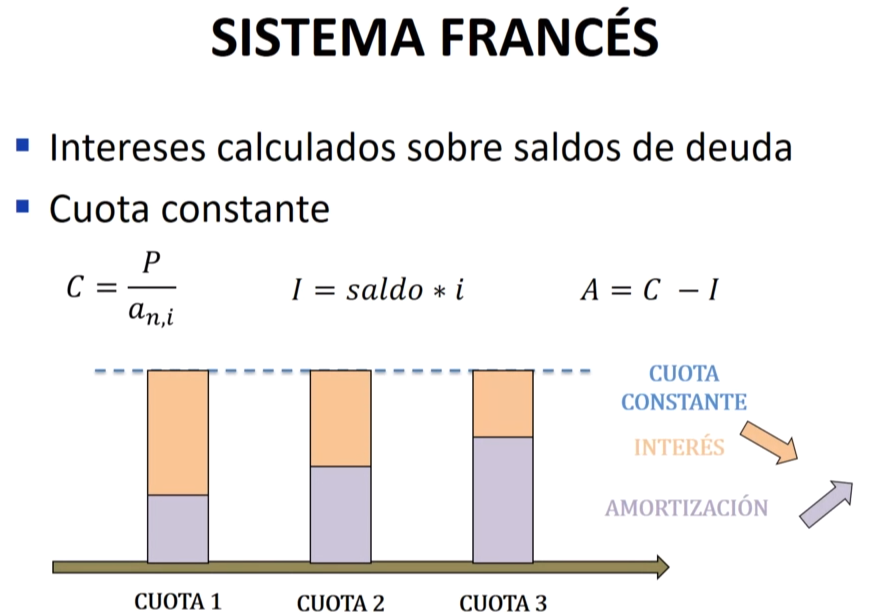
\includegraphics[width=0.7\linewidth]{fig/sist_frances.png}
	\caption{El valor presente a cuotas futuras el la deuda con el banco. Es el más usado para prestamos personales. Son anualidades, por ende $a_{n,i}$ de la figura es el factor anualidad.}
	\label{fig:sist_frances}
\end{figure}

\begin{figure}
	\centering
	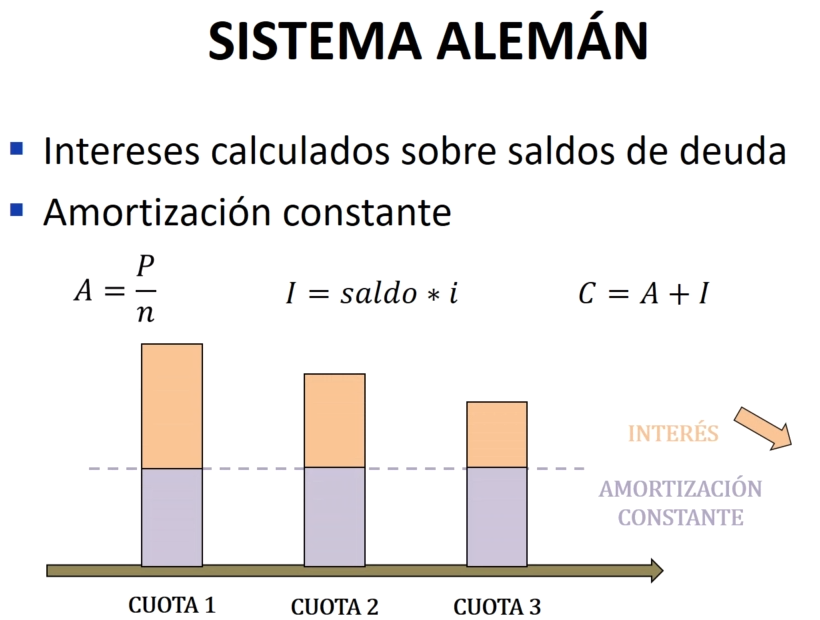
\includegraphics[width=0.7\linewidth]{fig/sist_aleman.png}
	\caption{La amortización del préstamo es constante, y como el saldo de deuda baja entonces los intereses también van a bajar. Más usado para empresas. }
	\label{fig:sist_aleman}
\end{figure}


\begin{figure}
	\centering
	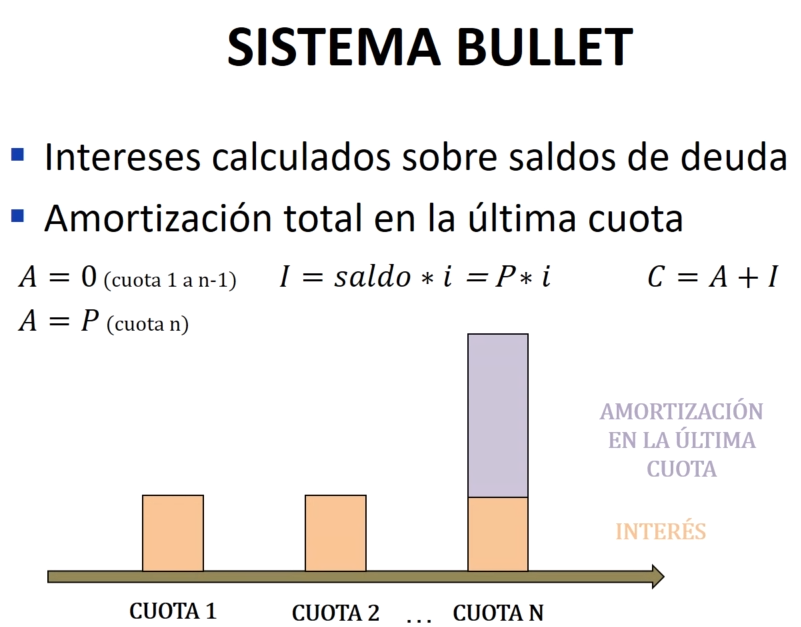
\includegraphics[width=0.7\linewidth]{fig/sist_bullet.png}
	\caption{La amortización se paga al final. Común para }
	\label{fig:sit_bullet}
\end{figure}

\begin{figure}
	\centering
	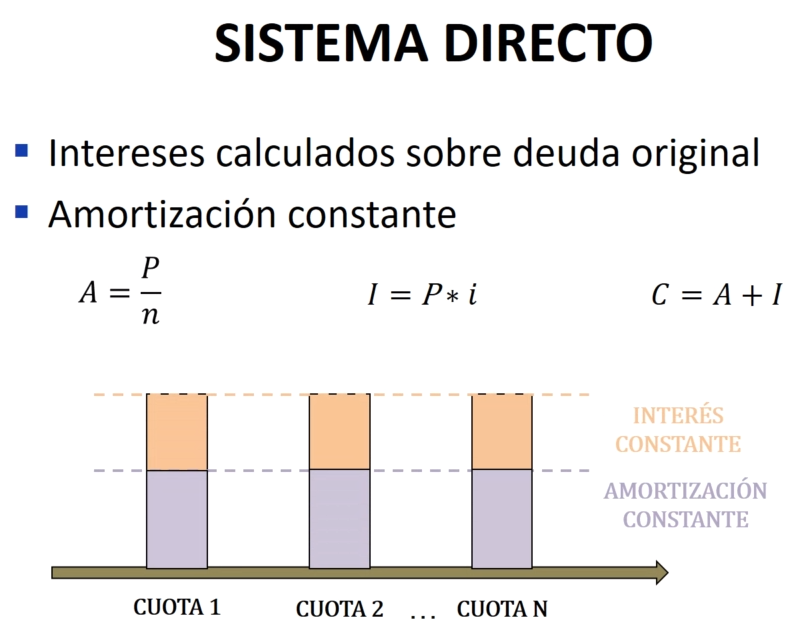
\includegraphics[width=0.7\linewidth]{fig/sit_directo.png}
	\caption{Sistema más marginal. El préstamo es más caro para el que recibe el préstamo porque los intereses se pagan sobre la deuda original}
	\label{fig:sit_directo}
\end{figure}


\section{Evaluación de proyectos}

\subsection{Flujo de caja}
El flujo de caja se hace \textbf{sin costos hundidos}. El flujo de caja refleja hecho irrefutables. Los beneficios en cambio no son concretos, pueden variar en función de como amortizas.

\subsection{Métodos de evaluación}

\begin{itemize}
	\item Valor: VAN/VPN/VNA
	\item Rendimiento: TIR, TER
	\item Recupero (t): PRS, PRC (periodo de recuperación)
\end{itemize}

\subsubsection{Valor actual neto (VAN)}

\[
	VAN = -I + P = \sum_{j=0}^n \frac{FC_j}{(1+i)^j}
\]
donde $I$ es el valor presente del costo del proyecto (habitualmente, la inversión inicial) y $P$ es el valor presente de los futuros flujos de caja del proyecto.

Si el VAN es positivo entonces hay un remanente de dinero después del proyecto que va al bolsillo. Si es cero entonces no se pierde ni gana dinero con el proyecto. Si es negativo entonces te conviene invertir a la tasa de interés usada para el VAN para no perder plata con el proyecto.

 \subsubsection{Tasa interna de retorno (TIR)}

 La TIR es la tasa de descuento $i$ que hace que el VAN del proyecto se haga cero, es decir, para cuando $P=I$.

 La TIR se compara con el costo del capital, que es lo que sacrifica el inversor de ganar en su mejor alternativa por decidirse a hacer la inversión. Esa tasa mínima se llama TREMA, \textbf{tasa requerida mínima atractiva} para el inversor. 
 
 La TIR es única para un proyecto con flujo de fondos simples. PAra proyectos complejos pueden haber varios TIR y conviene otro método de evaluación.

 \subsubsection{Resúmen de VAN y la TIR}
El VAN es propia del inversor ya que diferentes inversores pueden reducir costos con know-how de proyectos. En cambio la TIR es la misma para todo inversor de un proyecto.


\subsubsection{Tasa externa de retorno (TER)}

Para cuando hay más de una TIR se usa el método de la TER. La técnica consiste en calcular ek VP de todos los egresos y el VF de todos los ingresos, es decir: se agrupan todos los egresos al comienzo del proyecto en un gasto, y se agrupan los ingresos como un ingreso al final del proyecto.

No soluciona el problema de diferencia de escalas, es decir, no diferencia entre un proyecto con un VAN de 10\$ y uno con VAN de 10 millones \$.

El periodo de repago nos dice dentro cuanto tiempo se recupera la plata. Ayuda controlar riesgos asociados con la incertidumbre de los flujos de caja futuros. Útil en un país como Argentina donde un inversor tal vez no está tan cómodo esperando 10 años para recuperar su plata.


\begin{figure}
	\centering
	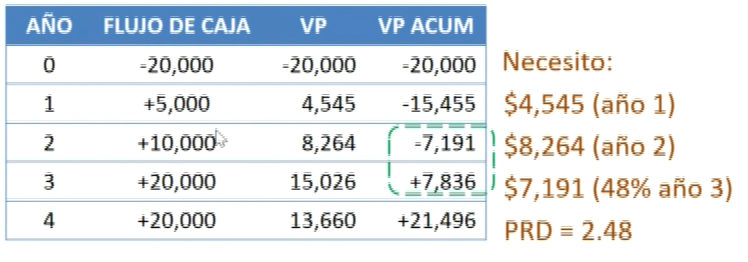
\includegraphics[width=0.9\linewidth]{fig/ej_periodoRepago.png}
	\caption{Ejemplo de un cálculo de Periodo de Repago (PRD) interpolando linealmente para obtener $t$.}
	\label{fig:periodoRepagoEjemplo}
\end{figure}

\subsection{Valor Anual Equivalente}
El VAE es una renta anual (anualidad) de flujos de caja equivalente a todos los ingresos y egreso, evaluados a la tasa de descuento.
\[
	VAE = VAN / factor(n,i)
\]
Donde el factor (de anualidad) es calculado según visto en la sección de anualidades. Sigue la regla de aceptación del VAN.

\subsection{Tasa de descuento}

La tasa de descuento se utiliza para determinar el valor presente de los flujos que generará un proyecto. Representa la rentabilidad mínima que debe exigirse a la inversión por renunciar a un uso alternativo de riesgo similar.

LA tasa de descuento visto desde el valor tiempo del dinero es la tasa de interés $i$ que hace al tomador de decisiones indiferente entre \$1 hoy y $\$(1+i)$ al final de un periodo.

La tasa de descuento para cual uno es indiferente se conoce como el costo oportunidad del dinero.

La tasa de descuento es muy importante para la evaluación de proyectos. Decide el costo del capital y por ende el VAN y TIR de un proyecto.

La tasa de descuento depende de como la empresa se financia de deudas (antes de impuestos) o recurso propios.


\section{Construcción del flujo de caja del proyecto}

Se construye a partir de los movimientos de caja del proyecto en el tiempo.

La forma más típica de modelar los flujos es ubicar un egreso en tiempo 0 y luego ubicar flujos ingresantes durante el \textbf{horizonte de proyecto}


\subsection{Cuadro de gastos o resultados}

\begin{table}[h]
	\centering
	\begin{tabular}{|l|} \hline
		+ Ingresos por ventas \\
		- Costos variables (``de ventas") \\ \hline
		= Utilidad bruta \\
		- Costos fijos (``Administración y ventas") \\ \hline
		= EBITDA \\
		- Amortizaciones \\ \hline
		= EBIT \\
		- Intereses \\ \hline
		= EBT \\
		- Impuestos a las ganacias
		\\ \hline
		= Utilidad Neta\\ \hline
	\end{tabular}
\caption{Cuadro de resultados}
\end{table}

\subsection{Costos de oportunidad}

Son costos que aparecen de manera no explicita. Una situación donde aparece el costo de oportunidad:

Para instalar una nueva linea de producción, la empresa B deberá utilizar un galpón propio, que hoy se alquila a un tercero percibiendo \$100.000 por mes.

\begin{itemize}
	\item Sin proyecto: +\$100.000 ingresos
	\item Con proyecto: El galpón se utiliza y se deja de facturar el alquiler. Se perdió la oportunidad de seguir facturando, por ende hay un costo de oportunidad de \$100.000
\end{itemize}

\subsection{Costos hundidos}

Son aquellos costos que resultan comunes a todas las alternativas. Se incurren sin importar la decisión. \textbf{No tiene sentido incluirlos en el análisis.}

El típico ejemplo de un costo hundido es un estudio de mercado. Se debe incurrir para poder empezar a formular una decisión!

\subsection{Valor terminal}
Al término del horizonte de planificación se hace un corte artificial con fines de evaluación. Ya no se consideran más ingresos y la planta deja de operar y se venden todos los activos. La suposición produce un flujo de efectivo extra en el último año.

Se debe suponer un valor de liquidación para los activos (máquinas, terreno, planta, etc.).

Se puede suponer también que la planta sigue operando con un flujo a perpetuidad y calcular el valor presente.

\subsection{Capital de trabajo}

Inversión que sirve para financiar los desfases que normalmente se producirán entre la generación de los ingresos y la ocurrencia de los egresos.

Puede estar compuesto de inversiones y recuperos intermedios de capital de trabajo. por ejemplo:

\begin{itemize}
	\item Productos estacionales
	\item Proyectos con curva de arranque
\end{itemize}

\begin{table}[h]
	\centering
	\begin{tabular}{|l|} \hline
		- Caja operativas \\
		- Créditos a clientes \\
		- Inventarios (MP, PP, PT) \\ \hline
		+ Deudas con proveedores    \\ \hline
		= Capital de trabajo operativo \\ \hline
	\end{tabular}
\caption{Cálculo de capital de trabajo operativo}
\end{table}




\begin{figure}[htb]
	\centering
	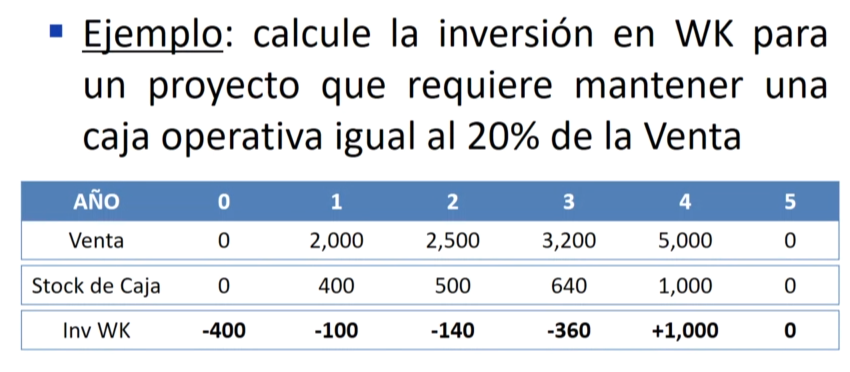
\includegraphics[width=1\linewidth]{fig/working_capital_example.png}
	\caption{}
	\label{fig:working_capital_example}
\end{figure}



\subsection{Costo financiero total (CFT)}

Es el costo efectivo de la financiación. Si no hay pagos extraordinarios ni comisiones es igual a la TEA.

\[
	CFT =  1 + (1+TIR)^{m}
\]




\end{document}
